\chapter{Arquitetura}
\label{cap:arquitetura}

\section{Microsserviços}

    O VuMoS foi implementado utilizando uma arquitetura modular de microsserviços, para que ele possa ser facilmente estendido e modificado no futuro caso necessário, e também para proporcionar uma maior facilidade de desenvolvimento de cada um dos módulos.
    
    \begin{figure}
        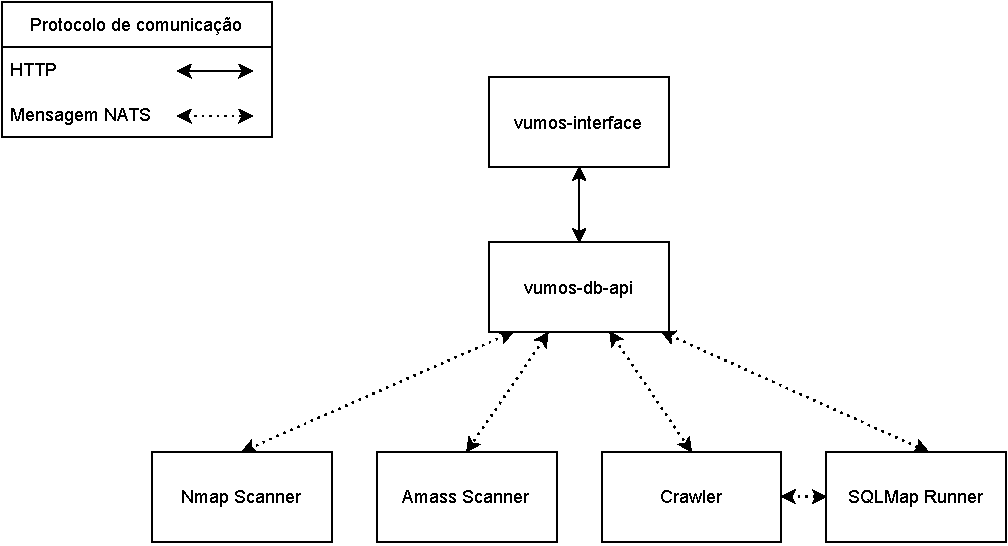
\includegraphics[scale=0.8]{figuras/vumos-Microservices.pdf}
        \caption{Diagrama de comunicação dos microsserviços.\label{fig:microservices}}
    \end{figure}
    
    Como pode ser visto em \ref{fig:microservices}, cada um dos 
    
    \subsection{NATS}
    
    Foi escolhido o \cite{NATS} como o sistema de mensageria da aplicação, principalmente devido a sua escalabilidade, simplicidade e performance. 
    
    
    
    \subsection{PostgreSQL}
    \subsection{Módulos}
        
        O sistema foi projetado de 
        
        \begin{figure}
            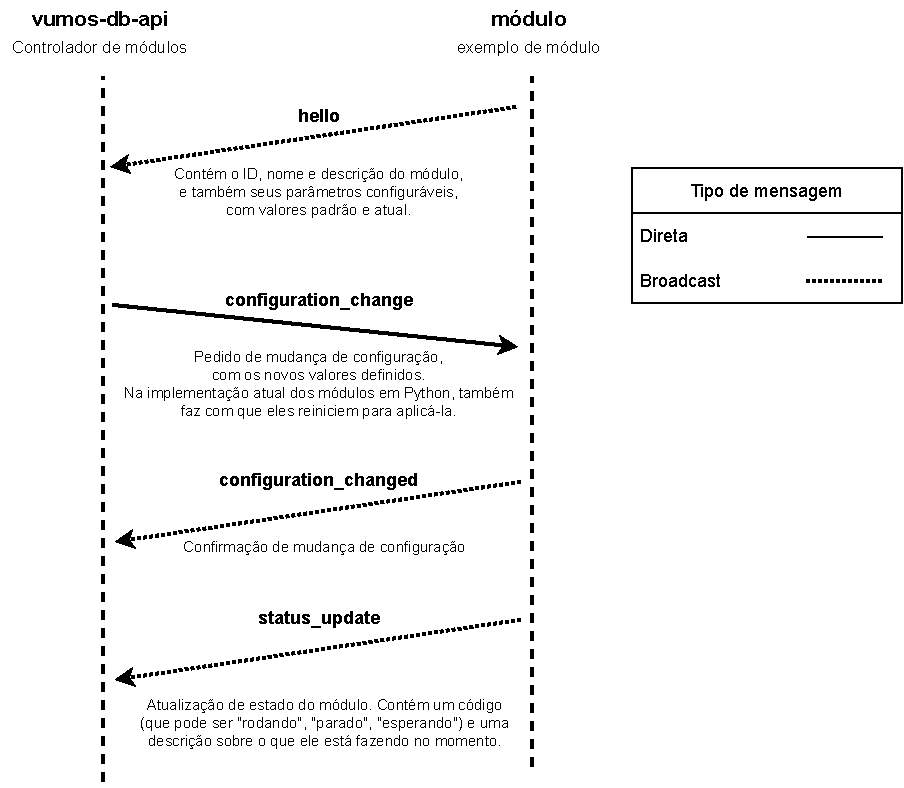
\includegraphics[scale=0.8]{figuras/vumos-module-communication.drawio.pdf}
            \caption{Diagrama de troca de mensagens entre um módulo e o gerenciador vumos-db-api.\label{fig:microservices}}
        \end{figure}
        
        % TODO: falar do startup (msg HELLO)
        % TODO: falar do VUMOS_ID
        % TODO: falar do vumos.py (a biblioteca em python)
            % TODO: falar do SQLite dentro de cada um, e do getconfig
            % TODO: falar do asyncio e do subprocess
        \subsubsection{Amass Scanner}
        \subsubsection{Nmap Scanner}
        \subsubsection{Crawler}
        \subsubsection{SQLMap Runner}
            % TODO: falar do threadpool
    
    \subsection{vumos-db-api}
    \subsection{vumos-interface}
    

\section{Orquestração}
    
    % TODO: falar das networks 
    \subsection{Produção}
    O VuMoS foi colocado em produção em http://vumos.hackersdobem.sti.usp.br/ e já está atualmente escanenado os  

